%%%%%%%%%%%%%%%%%%%%%%%%%%%%%%%%%%%%%%%%%%%%%%%%%%%%%%%%%%%%%%%%%%%%%%%%%%%%%%%%
\documentclass[twocolumn]{revtex4}

%%%%%%%%%%%%%%%%%%%%%%%%%%%%%%%%%%%%%%%%%%%%%%%%%%%%%%%%%%%%%%%%%%%%%%%%%%%%%%%%
% Note that comments begin with a "%" and are not turned into text in the .pdf
% document.
%%%%%%%%%%%%%%%%%%%%%%%%%%%%%%%%%%%%%%%%%%%%%%%%%%%%%%%%%%%%%%%%%%%%%%%%%%%%%%%%

%%%%%%%%%%%%%%%%%%%%%%%%%%%%%%%%%%%%%%%%%%%%%%%%%%%%%%%%%%%%%%%%%%%%%%%%%%%%%%%%
% Include some extra packages.
%%%%%%%%%%%%%%%%%%%%%%%%%%%%%%%%%%%%%%%%%%%%%%%%%%%%%%%%%%%%%%%%%%%%%%%%%%%%%%%%
\usepackage[]{graphicx}
%%%%%%%%%%%%%%%%%%%%%%%%%%%%%%%%%%%%%%%%%%%%%%%%%%%%%%%%%%%%%%%%%%%%%%%%%%%%%%%%

%%%%%%%%%%%%%%%%%%%%%%%%%%%%%%%%%%%%%%%%%%%%%%%%%%%%%%%%%%%%%%%%%%%%%%%%%%%%%%%%
\begin{document}

%%%%%%%%%%%%%%%%%%%%%%%%%%%%%%%%%%%%%%%%%%%%%%%%%%%%%%%%%%%%%%%%%%%%%%%%%%%%%%%%
\title{Final project - Can you escape a velociraptor if you get a head start?}

\author{Nico Carello}
\affiliation{Siena College, Loudonville, NY}

\date{\today}

\begin{abstract}
    The point of this project is to see if a raptor will catch you after you have a 30 meter head start and it has a chance of biting you when it is one meter behind you. The raptor travels at 18 m/s and you travel at 3 m/s. In order to do this we will use python to make a histogram and calculate when, where, and if the raptor gets you. The results: you ran for  about 2 seconds and 36 meters when it is one meter behind you and you have about a 60 percent chance of escaping. 
\end{abstract}

\maketitle
%%%%%%%%%%%%%%%%%%%%%%%%%%%%%%%%%%%%%%%%%%%%%%%%%%%%%%%%%%%%%%%%%%%%%%%%%%%%%%%%

%%%%%%%%%%%%%%%%%%%%%%%%%%%%%%%%%%%%%%%%%%%%%%%%%%%%%%%%%%%%%%%%%%%%%%%%%%%%%%%%
\section{Motivation}
%%%%%%%%%%%%%%%%%%%%%%%%%%%%%%%%%%%%%%%%%%%%%%%%%%%%%%%%%%%%%%%%%%%%%%%%%%%%%%%%
\subsection{Problem 1:} If you run at 3 m/s, a raptor runs at 18 m/s, and you have a 30 meter head start make a position vs time graph for you and the raptor.

\subsection{Problem 2:} Calculate when and where the raptor will catch you.

\subsection{Problem 3:} Calculate when it is close enough to bite you.

\subsection{Problem 4:} If you are one meter in front of the raptor and it has three chances of 20, 15, and 7 percent to get you, calculate the probability of you getting away.

\section{Algorithms and equations} 

\subsection{Problem 1:}
To solve problem 1 all you need to do is plot the lines of the human and raptor. You take the speeds of each entity and multiply it by the integers from zero to ten, this is time. The human will have a 30 meter head start, so I just added 30 to the formula.
	$$ RaptorPosition = RaptorSpeed * time $$
	$$ HumanPosition = HumanSpeed * time +30$$
	
\subsection{Problem 2:} I defined a function that found when and where the raptor catches the human. Using a for loop all times were looped through the equations for human and raptor positions. If the raptor position equals the human position return the time and location at that instant. This time and location is then printed to the screen.

\subsection{Problem 3:} The time and positon that the raptor can bite you is found by subtracting the raptor position from the human position. This function If that value is less than or equal to 1 then it is close enough to attack you.
$$ HumanPosition - RaptorPosition <= 1$$

\subsection{Problem 4:} Generate 3 different random integers between 0 and 100. Since the first chance that it bites you is 20, if the first number is less than 20 then it will bite you. The raptor has two more chances except they are 15 and 7 percent chances, respectively. If it is not successful after the third time then you get away. The probability of this is calculated by dividing the number of successful escapes in a range by 1000 and then multiplying by 100.
$$Probability = (success/1000) * 100$$

\section{Plots}
On the graphs the point where the lines cross each other is the point where the raptor catches up to you.
\begin{figure}[h]
	\centering
	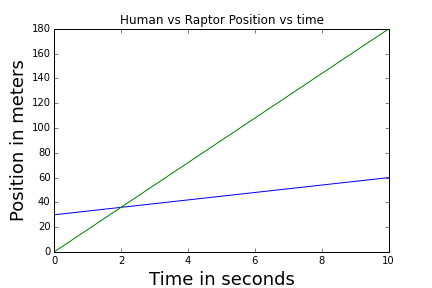
\includegraphics[width=0.45\textwidth]{RaptorVHuman.png}
	\caption{This is the graph \label{fig:Graph}}
\end{figure}

\begin{figure}[h]
	\centering
	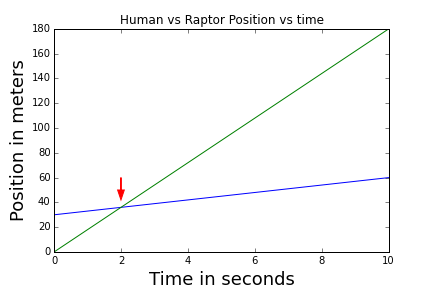
\includegraphics[width=0.45\textwidth]{Arrow.png}
	\caption{This is the graph with the arrow. \label{fig:Graph}}
\end{figure}
%%%%%%%%%%%%%%%%%%%%%%%%%%%%%%%%%%%%%%%%%%%%%%%%%%%%%%%%%%%%%%%%%%%%%%%%%%%%%%%%

%%%%%%%%%%%%%%%%%%%%%%%%%%%%%%%%%%%%%%%%%%%%%%%%%%%%%%%%%%%%%%%%%%%%%%%%%%%%%%%%

%%%%%%%%%%%%%%%%%%%%%%%%%%%%%%%%%%%%%%%%%%%%%%%%%%%%%%%%%%%%%%%%%%%%%%%%%%%%%%%%
\end{document}
%%%%%%%%%%%%%%%%%%%%%%%%%%%%%%%%%%%%%%%%%%%%%%%%%%%%%%%%%%%%%%%%%%%%%%%%%%%%%%%%
